\chapter{Вращения, спиноры и цветовая симметрия}

\section{Вращения как группа}

Вращения пространства — это симметрии, и они действуют на многие типы объектов. Они действуют на твердые тела, на векторы скорости, на векторные поля и на квантовые состояния. Обычный вектор — самый простой объект, с которого можно начать, потому что его преобразование можно наглядно представить.

Вращения можно и комбинировать. Поверните объект вокруг одной оси на некоторый угол, а затем вокруг второй оси на другой угол. Конечная ориентация эквивалентна одному вращению вокруг некоторой третьей оси на некоторый третий угол. Следовательно, произведение двух вращений есть снова вращение.

Это произведение — операция над преобразованиями, а не сложение двух векторов осей. Первое вращение изменяет объект, на который действует второе. Если сначала выполняется \(R_1\), а затем \(R_2\), то составная операция записывается как \(R_2R_1\). Она сама является некоторым \(R_3\), хотя нахождение оси и угла для \(R_3\) может быть неудобным. Эта замкнутость относительно композиции — первая причина рассматривать вращения как группу, а не просто как список геометрических движений.

Полезно сначала геометрически описать одно вращение. Выберем единичный вектор \(\hat{\boldsymbol n}\) вдоль оси вращения и угол \(\theta\). Мы используем правило правой руки. Левостороннее вращение на \(\theta\) можно столь же хорошо записать как правостороннее вращение на \(-\theta\) или как правостороннее вращение вокруг \(-\hat{\boldsymbol n}\).

\begin{figure}[htbp]
\centering
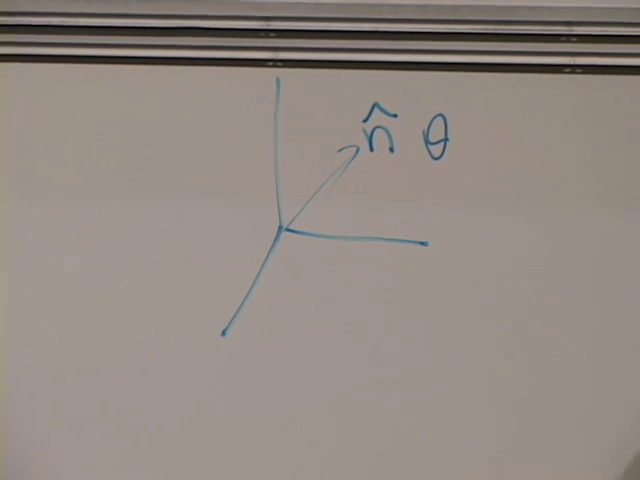
\includegraphics[width=0.58\textwidth]{lecture_03_figure_02.png}
\caption{Ось \(\hat{\boldsymbol n}\) и угол \(\theta\) задают пространственное вращение.}
\lectureframe{00:02:34}
\end{figure}

Направление на единичной сфере требует двух параметров, например долготы и широты. Угол поворота вокруг этого направления дает третий. Поэтому вращения образуют трехпараметрическое семейство. Мы пока не будем беспокоиться о глобальных отождествлениях, возникающих из-за углов, отличающихся на \(2\pi\); здесь важен именно локальный подсчет параметров.

Описание через ось и угол содержит некоторую избыточность. Если обратить ось и одновременно изменить знак угла, получится та же операция, а достаточно большие углы можно сводить по модулю полного оборота. Ничто из этого не меняет того факта, что вблизи единичного элемента вращение имеет три непрерывно изменяющихся параметра. Этот локальный счет позже будет сопоставлен с числом независимых параметров в матричном представлении.

Свойства группы теперь можно поочередно проверить:
\begin{enumerate}
\item \emph{Замкнутость.} Последовательное выполнение двух вращений дает другое вращение.
\item \emph{Единичный элемент.} Ничего не делать — это тождественное вращение.
\item \emph{Обратный элемент.} Вращение на \(\theta\) вокруг \(\hat{\boldsymbol n}\) компенсируется вращением на \(-\theta\) вокруг той же оси.
\item \emph{Ассоциативность.} Для трех последовательных вращений выполняется
\[
(R_1R_2)R_3=R_1(R_2R_3).
\]
\end{enumerate}

Вращения некоммутативны. Вращение вокруг оси \(x\), за которым следует вращение вокруг оси \(y\), вообще говоря, приводит к иной ориентации, чем те же две операции в обратном порядке:
\begin{equation}
R_x(\alpha)R_y(\beta)\ne R_y(\beta)R_x(\alpha).
\end{equation}
Различие становится величиной второго порядка, когда оба угла очень малы, поэтому бесконечно малые вращения могут казаться почти коммутативными. Тем не менее полная группа неабелева.

Некоммутативность можно проверить и без всяких уравнений. Возьмите книгу или коробку, отметьте одну грань как переднюю и поверните предмет на девяносто градусов вокруг оси \(x\), а затем на девяносто градусов вокруг оси \(y\). Верните его в исходную ориентацию и поменяйте порядок. Отмеченная грань окажется направленной иначе. Для малых углов расхождение заметить труднее, но оно не исчезло; оно начинается с произведения двух малых углов.

\begin{classroomqa}
\audiencequestion{Эти вращения последовательные, а не одновременные?\lecturetimestamp{00:04:45}}
\lecturerresponse{Да. Умножение в группе означает, что одна операция выполняется после другой. Именно порядок этих последовательных вращений может не коммутировать.}
\end{classroomqa}

Это наша первая неабелева группа. Ее дальнейшее применение связано не с цветом обычного предмета, а с красным, зеленым и синим цветовыми состояниями кварка. Это внутренняя система с тремя состояниями, и ее нетривиальные преобразования смешивают три цвета. Обычные вращения дают знакомую модель того, как непрерывная группа действует через матрицы.

Сама по себе группа абстрактна. Чтобы использовать ее в физике, надо указать, на каких объектах она действует. {Представление} сопоставляет каждому элементу группы оператор или матрицу так, что умножение элементов группы воспроизводится умножением сопоставленных матриц. Разные физические объекты могут нести разные представления одной и той же группы. Векторы, состояния со спином 1 и состояния со спином 1/2 дадут три примера.

\section{Трехмерное векторное представление}

Пусть обычный вектор имеет компоненты
\begin{equation}
\boldsymbol V=(V_x,V_y,V_z),\qquad V_i,\quad i=1,2,3.
\end{equation}
Можно вращать сам физический вектор, удерживая оси неподвижными, или вращать координатные оси, удерживая вектор неподвижным. Соглашения различаются, но в обоих описаниях компоненты смешиваются матрицей \(3\times3\). Для каждой пары ось–угол \((\hat{\boldsymbol n},\theta)\) запишем
\begin{equation}
V_i'=R_{ij}(\hat{\boldsymbol n},\theta)V_j,
\label{eq:l3-vector-rotation}
\end{equation}
где по повторяющемуся индексу производится суммирование.

Повторяющийся индекс \(j\) — фиктивный индекс. Уравнение~\eqref{eq:l3-vector-rotation} в явном виде означает
\begin{equation}
V_i'=R_{i1}V_1+R_{i2}V_2+R_{i3}V_3
\end{equation}
для каждой результирующей компоненты \(i\). Свободный индекс \(i\) указывает, какая компонента вычисляется; по повторяющемуся \(j\) ведется суммирование, и его можно переименовать, не меняя уравнения. Разделение этих двух ролей предотвращает большинство ошибок с индексами в рассуждении о сохранении длины.

\begin{figure}[htbp]
\centering
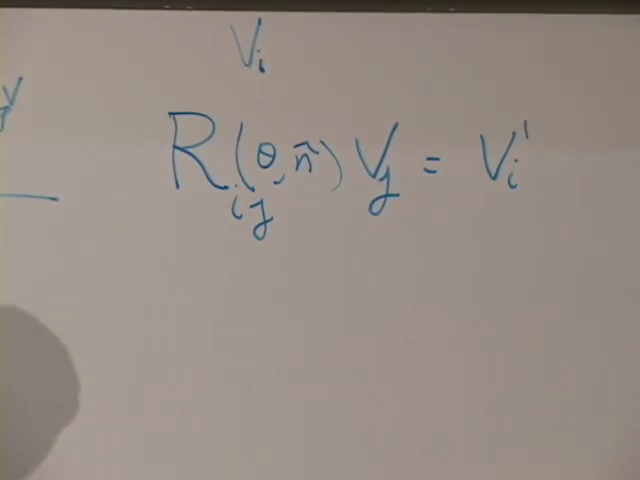
\includegraphics[width=0.68\textwidth]{lecture_03_figure_03.png}
\caption{Матрица вращения переводит исходные компоненты вектора в компоненты после поворота.}
\lectureframe{00:07:41}
\end{figure}

Настоящее вращение сохраняет длину. Пока и \(V_i\), и \(R_{ij}\) вещественны, поэтому
\begin{equation}
V_i'V_i'=V_iV_i
\end{equation}
для любого вектора. Чтобы выявить условие на матрицу, запишем то же преобразование с другими фиктивными индексами:
\begin{equation}
V_i'=R_{ij}V_j,\qquad V_i'=R_{ik}V_k.
\end{equation}
Перемножая и суммируя по \(i\), получаем
\begin{align}
V_i'V_i'
 &=R_{ij}V_jR_{ik}V_k\\
 &=R_{ij}R_{ik}V_jV_k.
\end{align}
Это равно \(V_jV_j\) при любом выборе \(V\) только в том случае, если
\begin{equation}
R_{ij}R_{ik}=\delta_{jk}.
\label{eq:l3-orthogonality-index}
\end{equation}
В матричной записи
\begin{equation}
R^TR=\boldsymbol 1,
\label{eq:l3-orthogonal}
\end{equation}
и, следовательно,
\begin{equation}
R^{-1}=R^T.
\end{equation}
Транспонирование просто меняет строки и столбцы местами.

Почему коэффициент должен быть равен \(\delta_{jk}\)? Символ Кронекера при суммировании полагает \(j=k\):
\begin{equation}
\delta_{jk}V_jV_k=V_1^2+V_2^2+V_3^2.
\end{equation}
Если бы \(R_{ij}R_{ik}\) отличалось от \(\delta_{jk}\), то длина менялась бы либо для некоторого направления, либо из-за некоторого перекрестного члена \(V_jV_k\). Поскольку равенство требуется для всякого возможного вектора, а не только для одного выбранного, сам этот матричный коэффициент должен совпадать с единичной матрицей.

Уравнение~\eqref{eq:l3-orthogonal} есть определяющее условие ортогональности для этого вещественного матричного представления. Умножение матриц воспроизводит таблицу умножения пространственных вращений. Это не единственное представление группы вращений; просто его легче всего наглядно представить.

Соотношение для обратной матрицы имеет непосредственный геометрический смысл. Вращение можно обратить, не решая нового матричного уравнения: достаточно поменять местами строки и столбцы. Если \(R_1\) и \(R_2\) представляют два вращения, то \(R_2R_1\) представляет их последовательное действие и снова является ортогональной матрицей. Тем самым матричные операции сохраняют ту же структуру замкнутости, единичного элемента, обратного элемента и ассоциативности, которая была установлена геометрически.

\section{Спин 1 и векторное представление}

Трехмерное представление действует и на квантовые состояния. У частицы со спином 1 возможны три проекции спина,
\begin{equation}
m=+1,\quad 0,\quad -1.
\end{equation}
Поэтому ее спиновое состояние представляет собой трехкомпонентный столбец амплитуд вероятности. Вращение частицы или изменение ориентации магнитного поля, используемого для задания оси спина, смешивает эти три амплитуды согласно трехмерному представлению группы вращений.

Число спиновых состояний подчиняется знакомому правилу \(2s+1\). Спин 0 имеет одно состояние, спин 1/2 — два, спин 1 — три, а спин 3/2 — четыре. Поэтому размерность вектора состояния зависит от спина. Одно и то же физическое вращение должно представляться матрицами разных размеров, когда оно действует в этих различных пространствах состояний.

Для частицы со спином 1 выберем базис
\begin{equation}
\lvert 1,+1\rangle,qquad
\lvert 1,0\rangle,qquad
\lvert 1,-1\rangle.
\end{equation}
Состояние имеет вид
\begin{equation}
\lvert\psi\rangle
=c_{+}\lvert1,+1\rangle+c_0\lvert1,0\rangle+c_{-}\lvert1,-1\rangle.
\end{equation}
Поворот установки не создает четвертого спинового состояния; он лишь смешивает между собой три коэффициента \(c_+,c_0,c_-\). Поэтому соответствующий оператор вращения должен быть матрицей \(3\times3\).

Для спина 1 это представление преобразуется так же, как обычный пространственный вектор. Именно в этом состоит точный смысл того, что частицу со спином 1 называют \emph{векторной частицей}: ее три спиновые амплитуды и три компоненты вектора подчиняются одному и тому же закону вращения. Квантовое состояние не нужно представлять как буквальную стрелку; утверждение относится к тому, как смешиваются его компоненты.

Это соответствие не случайно. Трёхвектор и состояние со спином 1 несут эквивалентные трёхмерные представления группы вращений. Слова emph{векторная частица} кратко выражают это свойство преобразования. Они не утверждают, что квантовое состояние поляризации — это крошечная жёсткая стрелка, скрытая внутри частицы.

\section{Дискретные и непрерывные симметрии}

Прежде чем перейти к спину 1/2, полезно различить два широких класса групп. Простое дискретное пример даёт отражение. Есть тождественный элемент и есть отражение \(P\); либо отражение происходит, либо нет. Напротив, фаза
\begin{equation}
e^{i\phi}
\end{equation}
непрерывно зависит от \(\phi\), а пространственное вращение непрерывно зависит от своей оси и угла. Такие непрерывные группы называются \emph{группами Ли}, в честь Софуса Ли; его фамилия произносится \emph{Ли}. Основное внимание будет уделено непрерывным симметриям, хотя дискретные симметрии также остаются важными.

Для двухэлементной группы отражений,
\begin{equation}
P^2=1.
\end{equation}
Между \(1\) и \(P\) нет непрерывно регулируемой степени отражения. С фазовой группой дело обстоит иначе: между \(e^{i\phi_1}\) и \(e^{i\phi_2}\) лежит непрерывное множество других фаз. Пространственные вращения обладают тем же непрерывным характером, но, в отличие от \(U(1)\), они неабелевы.

Спин 0 даёт простейшее представление группы вращений. Состояние со спином 0 не изменяется при любом вращении, поэтому каждый элемент группы представляется одномерной единицей:
\begin{equation}
D^{(0)}(R)=1.
\end{equation}
Сама группа по-прежнему содержит бесконечно много вращений; тривиальным является именно представление на состоянии со спином 0.

Это различие между группой и одним из её представлений существенно. Группа вращений не сводится к группе из одного элемента всякий раз, когда она действует на скаляр. Напротив, каждый её элемент на этом конкретном скалярном состоянии представляется одним и тем же числом \(1\).

\section{Общее состояние со спином 1/2}

Система со спином 1/2 имеет два базисных состояния. Относительно выбранной оси \(z\),
\begin{equation}
\lvert\uparrow\rangle=
\begin{pmatrix}1\\0\end{pmatrix},
\qquad
\lvert\downarrow\rangle=
\begin{pmatrix}0\\1\end{pmatrix}.
\end{equation}
Общее состояние есть двухкомпонентный спинор,
\begin{equation}
\lvert\psi\rangle=
\begin{pmatrix}\alpha_1\\\alpha_2\end{pmatrix},
\qquad
|\alpha_1|^2+|\alpha_2|^2=1.
\label{eq:l3-spinor}
\end{equation}
Его компоненты комплексны. Выбор \((\alpha_1,\alpha_2)=(1,0)\) соответствует спину вверх, а \((0,1)\) — спину вниз. Общая нормированная комбинация описывает спин, поляризованный вдоль некоторого другого направления.

Слова emph{вверх} и emph{вниз} имеют смысл только после выбора оси. Здесь этой осью является \(z\). Другой оси измерения соответствует другая пара базисных состояний, и состояние, которое вдоль одной оси определённо является верхним, в другом базисе, как правило, выглядит как суперпозиция. При вращении физического спина или при вращении осей отсчёта коэффициенты изменяются соответствующим образом.

Две комплексные амплитуды содержат 4 вещественных параметра. Нормировка устраняет один, а физически несущественная общая фаза устраняет ещё один, так что остаются два вещественных параметра. Это ровно то число, которое нужно, чтобы задать направление на сфере. Нам не нужно выводить явное соответствие между \((\alpha_1,\alpha_2)\) и этим направлением, чтобы изучать вращения.

Общая фаза устраняется, потому что
\begin{equation}
\begin{pmatrix}\alpha_1\\\alpha_2\end{pmatrix}
\quad\hbox{and}\quad
e^{i\chi}
\begin{pmatrix}\alpha_1\\\alpha_2\end{pmatrix}
\end{equation}
представляют один и тот же физический луч. Нормировка фиксирует полную вероятность, а не направление в обычном евклидовом пространстве. После обеих этих идентификаций оставшиеся два параметра можно рассматривать как полярный и азимутальный углы направления поляризации спина.

Когда спин вращается, его состояние становится
\begin{equation}
\alpha_i'=U_{ij}\alpha_j,
\qquad
\begin{pmatrix}\alpha_1'\\\alpha_2'\end{pmatrix}
=
\begin{pmatrix}
U_{11}&U_{12}\\
U_{21}&U_{22}
\end{pmatrix}
\begin{pmatrix}\alpha_1\\\alpha_2\end{pmatrix}.
\label{eq:l3-spinor-transform}
\end{equation}
Следовательно, пространственные вращения обладают двумерным матричным представлением, действующим на спиноры. В этом представлении имеется глобальная двузначность, обсуждение которой мы пока отложим; локально матрицы обладают свойствами преобразования, необходимыми далее.

Преобразованная пара \((\alpha_1',\alpha_2')\) снова должна быть допустимым квантовым состоянием. Поэтому первый вопрос о \(U\) — не его явная формула через ось и угол, а условие, при котором оно сохраняет нормировку любого исходного спинора.

\section{Сохранение вероятности и унитарные матрицы}

Вращение должно переводить нормированное состояние в другое нормированное состояние:
\begin{equation}
\alpha_i^*\alpha_i=\alpha_i'^*\alpha_i'=1.
\end{equation}
Подставляя уравнение~\eqref{eq:l3-spinor-transform},
\begin{align}
\alpha_i'^*\alpha_i'
 &=(U_{ij}\alpha_j)^*(U_{ik}\alpha_k)\\
 &=\alpha_j^*U_{ij}^*U_{ik}\alpha_k.
\end{align}
Поэтому аналог условия для вещественного вектора имеет вид
\begin{equation}
(U^T)^*U=\boldsymbol 1.
\end{equation}
Транспонирование с последующим комплексным сопряжением даёт эрмитово сопряжение,
\begin{equation}
U^\dagger=(U^T)^*,
\end{equation}
так что условие сохранения нормировки таково:
\begin{equation}
U^\dagger U=\boldsymbol 1.
\label{eq:l3-unitarity}
\end{equation}

Дополнительное комплексное сопряжение — единственное существенное изменение по сравнению с вычислением для вещественного вектора. Для вещественного вектора \(V_iV_i\) есть длина. Для спинора \(\alpha_i^*\alpha_i\) есть вероятность. Комплексное сопряжение необходимо, чтобы сделать эту вероятность вещественной и неотрицательной, поэтому транспонирование заменяется эрмитовым сопряжением.

Уравнение~\eqref{eq:l3-unitarity} также сразу даёт обратную матрицу:
\begin{equation}
U^{-1}=U^\dagger.
\end{equation}
Поэтому обратное вращение сохраняет ту же вероятностную норму. Как и для обычных матриц вращения, произведения унитарных матриц остаются унитарными, так что представление согласовано с групповым умножением.

\begin{figure}[htbp]
\centering
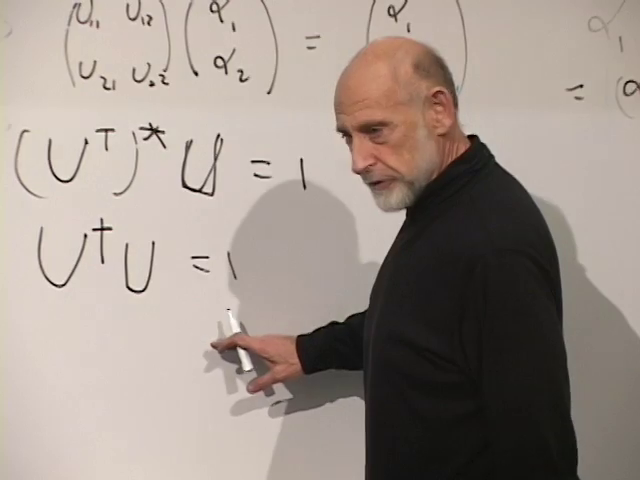
\includegraphics[width=0.62\textwidth]{lecture_03_figure_04.png}
\caption{Матрица вращения спинора удовлетворяет условию \(U^\dagger U=\boldsymbol 1\).}
\lectureframe{00:27:41}
\end{figure}

Матрицы, удовлетворяющие уравнению~\eqref{eq:l3-unitarity}, унитарны. Общая комплексная матрица \(2\times2\) содержит 8 вещественных параметров. Унитарность есть матричное уравнение \(2\times2\), дающее 4 независимых вещественных ограничения, так что остаются 4 параметра. Пространственное вращение имеет только 3. Нужно ещё одно ограничение, чтобы выделить спинорное представление вращений из всего \(U(2)\).

Эти 4 ограничения можно увидеть и иначе, если рассматривать два столбца \(U\) как два комплексных вектора. Каждый столбец должен иметь единичную норму, что даёт 2 вещественных условия, а столбцы должны быть ортогональны, что даёт одно комплексное, или 2 вещественных, условия. Итого получается 4. Оставшийся четвёртый параметр в \(U(2)\) окажется общей фазой детерминанта, а не новым пространственным вращением.

\section{Детерминант, равный единице, и \texorpdfstring{\(SU(2)\)}{SU(2)}}

Дополнительное условие таково:
\begin{equation}
\det U=1.
\label{eq:l3-det-one}
\end{equation}
Оно совместимо с групповым умножением, поскольку
\begin{equation}
\det(AB)=\det A\,\det B.
\end{equation}
Произведение двух унитарных матриц с детерминантом, равным 1, снова имеет детерминант 1, и единичная матрица имеет детерминант 1. Эти матрицы образуют замкнутую подгруппу.

Обратный элемент также принадлежит этой подгруппе. Если \(\det U=1\), то
\begin{equation}
\det U^{-1}=\frac{1}{\det U}=1.
\end{equation}
Следовательно, наложение условия det=1 не устраняет единичный элемент, не нарушает замкнутость и не лишает группу обратных элементов. Оно последовательно выделяет группу с одним непрерывным параметром меньше.

Сама по себе унитарность влечёт
\begin{equation}
\det(U^\dagger U)=
(\det U)^*\det U
=|\det U|^2=1.
\end{equation}
Она не вынуждает \(\det U\) быть равным \(+1\) или \(-1\). Детерминант общей унитарной матрицы может быть любой фазой:
\begin{equation}
\det U=e^{i\phi},
\qquad
\det U^\dagger=e^{-i\phi}.
\end{equation}
Условие~\eqref{eq:l3-det-one} фиксирует эту в противном случае свободную фазу и устраняет один вещественный параметр.

\begin{classroomqa}
\audiencequestion{Следует ли из \(U^\dagger U=\boldsymbol 1\), без условия единичного детерминанта, что \(\det U^\dagger\) должно равняться \(\det U\) или принимать только значения \(+1\) или \(-1\)?\lecturetimestamp{00:31:21}}
\lecturerresponse{Нет. Эти два детерминанта комплексно сопряжены. Они могут быть равны \(e^{i\phi}\) и \(e^{-i\phi}\), произведение которых равно единице. Ограничение специальной унитарности затем фиксирует оба равными единице.}
\end{classroomqa}

Унитарные матрицы \(n\times n\) образуют \(U(n)\). При \(n=1\) унитарная матрица — это просто фаза \(e^{i\phi}\), что даёт \(U(1)\). Подгруппа с детерминантом, равным 1, есть \emph{специальная унитарная группа},
\begin{equation}
SU(n)=\{U\in U(n):\det U=1\}.
\end{equation}
На двухкомпонентный спинор действует \(SU(2)\), группа с 3 параметрами.

Обозначение отражает оба ограничения: \(U\) означает унитарность, тогда как \(S\) означает, что группа специальная, то есть с детерминантом 1. Такие специальные унитарные группы возникают вновь и вновь, потому что они сохраняют комплексное внутреннее произведение, исключая при этом независимую общую фазу, связанную с детерминантом.

Локально \(SU(2)\) имеет ту же алгебру вращений и ту же структуру умножения, которые нужны для вращения состояний со спином 1/2. Глобально нужно помнить об отложенной тонкости: \(SU(2)\) является двукратным накрытием обычной группы вращений \(SO(3)\), так что двум элементам \(SU(2)\) соответствует одно пространственное вращение. \editorialnote{Формулировка через двукратное накрытие точно выражает упомянутую, но не развитую в исходном тексте, двузначность.}

\section{Бесконечно малые вращения и матрицы Паули}

\begin{classroomqa}
\audiencequestion{Где в этой конструкции появляются спиновые матрицы, или матрицы Паули?\lecturetimestamp{00:33:16}}
\lecturerresponse{Они появляются, когда элемент группы берётся очень близким к единице, что соответствует вращению на очень малый угол. Они являются генераторами этих бесконечно малых вращений.}
\end{classroomqa}

Начнём с
\begin{equation}
U=\boldsymbol 1+\epsilon M+O(\epsilon^2),
\label{eq:l3-small-u-anti}
\end{equation}
где \(\epsilon\) вещественно и мало. Тогда
\begin{equation}
U^\dagger=\boldsymbol 1+\epsilon M^\dagger+O(\epsilon^2),
\end{equation}
и из унитарности следует
\begin{align}
U^\dagger U
 &=\boldsymbol 1+\epsilon(M^\dagger+M)+O(\epsilon^2).
\end{align}
В первом порядке,
\begin{equation}
M^\dagger=-M.
\end{equation}
Следовательно, матрица \(M\) в уравнении~\eqref{eq:l3-small-u-anti} антиэрмитова.

Сохраняются только члены, линейные по \(\epsilon\). Произведение \(\epsilon^2M^\dagger M\) отбрасывается, потому что оно имеет второй порядок. В этом и состоит преимущество работы вблизи единицы: нелинейные групповые условия превращаются в линейные условия на их генераторы.

Удобнее вынести множитель \(i\):
\begin{equation}
U=\boldsymbol 1+i\epsilon H+O(\epsilon^2).
\label{eq:l3-small-u-herm}
\end{equation}
При комплексном сопряжении \(i\) переходит в \(-i\), поэтому
\begin{equation}
U^\dagger=\boldsymbol 1-i\epsilon H^\dagger+O(\epsilon^2).
\end{equation}
Теперь
\begin{equation}
U^\dagger U
=\boldsymbol 1+i\epsilon(H-H^\dagger)+O(\epsilon^2),
\end{equation}
и унитарность в первом порядке требует
\begin{equation}
H^\dagger=H.
\end{equation}
Когда множитель \(i\) вынесен явно, генератор является эрмитовым.

Умножение на \(i\) не изменило допустимые бесконечно малые матрицы; оно лишь изменило соглашение, по которому называют генератор. В физике обычно выбирают эрмитовы генераторы, потому что их собственные значения вещественны и потому что соответствующие наблюдаемые, такие как момент импульса, эрмитовы.

Условие равенства определителя единице даёт бесследовость\editorialnote{В устном разложении определителя индексы на короткое время искажены. Исправленный линейный член — \(A_{11}+A_{22}=\operatorname{tr}A\); произведения внедиагональных элементов начинаются со второго порядка.}. Для малой матрицы \(2\times2\) \(A\),
\begin{equation}
\det(\boldsymbol 1+A)
=
\det
\begin{pmatrix}
1+A_{11}&A_{12}\\
A_{21}&1+A_{22}
\end{pmatrix}.
\end{equation}
Раскрывая определитель,
\begin{align}
\det(\boldsymbol 1+A)
 &=(1+A_{11})(1+A_{22})-A_{12}A_{21}\\
 &=1+A_{11}+A_{22}+O(A^2)\\
 &=1+\operatorname{tr}A+O(A^2).
\end{align}
Применяя это к \(A=i\epsilon H\),
\begin{equation}
\det U=1+i\epsilon\,\operatorname{tr}H+O(\epsilon^2).
\end{equation}
Следовательно, \(\det U=1\) требует
\begin{equation}
\operatorname{tr}H=0.
\end{equation}
Условие на след устраняет в точности генератор, пропорциональный единичной матрице. Общая эрмитова матрица \(2\times2\) имеет четыре вещественных параметра: два вещественных диагональных элемента и один комплексный внедиагональный элемент. Её след фиксирует одну вещественную комбинацию, оставляя три. Это соответствует трём осям, относительно которых можно совершить бесконечно малый пространственный поворот.

Таким образом, бесконечно малые генераторы \(SU(2)\) — это бесследовые эрмитовы матрицы \(2\times2\). Три матрицы Паули образуют базис:
\begin{equation}
\begin{aligned}
\sigma_x&=
\begin{pmatrix}0&1\\1&0\end{pmatrix},
&
\sigma_y&=
\begin{pmatrix}0&-i\\i&0\end{pmatrix},
\\[0.4em]
\sigma_z&=
\begin{pmatrix}1&0\\0&-1\end{pmatrix}.
\end{aligned}
\end{equation}
Любой генератор можно записать в виде
\begin{equation}
H=a_x\sigma_x+a_y\sigma_y+a_z\sigma_z.
\end{equation}
Малый поворот вокруг оси \(x\) выделяет \(\sigma_x\); поворот вокруг оси \(y\) — \(\sigma_y\); а поворот вокруг любой другой оси выделяет соответствующую линейную комбинацию. В единицах, где \(\hbar=1\), операторы спина имеют вид
\begin{equation}
S_i=\frac{\sigma_i}{2}.
\end{equation}

Например, оси, лежащей посередине между \(x\) и \(y\), соответствует генератор, пропорциональный
\begin{equation}
\frac{\sigma_x+\sigma_y}{\sqrt2}.
\end{equation}
Направление вектора коэффициентов \((a_x,a_y,a_z)\) задаёт ось поворота, тогда как его модуль вместе с \(\epsilon\) задаёт малый угол. В этом и состоит связь между спиновыми матрицами, встречающимися в коммутационных соотношениях для момента импульса, и операторами конечных поворотов. В частности,
\begin{equation}
[S_x,S_y]=iS_z
\end{equation}
а её циклические аналоги кодируют некоммутативность, уже увиденную геометрически. Стандартный конечный поворот получается экспоненцированием бесконечно малого генератора\editorialnote{Экспоненциальная формула конечного поворота представляет собой стандартное завершение бесконечно малого построения; в источнике выводятся только условия на генераторы и их базис из матриц Паули.},
\begin{equation}
U(\hat{\boldsymbol n},\theta)
=\exp\left(-\frac{i\theta}{2}\,
\hat{\boldsymbol n}\cdot\boldsymbol\sigma\right).
\end{equation}
\section{Трёхсостоянийное цветовое пространство}

Объединение представлений может подождать. Теперь мы оставим пространственный спин и вернёмся к цвету кварка. Кварк по-прежнему имеет спин 1/2, но его цвет — это независимая трёхсостоянийная степень свободы:
\begin{equation}
\lvert r\rangle,\qquad
\lvert g\rangle,\qquad
\lvert b\rangle.
\end{equation}
Общее цветовое состояние имеет вид
\begin{equation}
\begin{aligned}
\lvert q\rangle_{\mathrm{color}}
={}&
\alpha_r\lvert r\rangle
+\alpha_g\lvert g\rangle
+\alpha_b\lvert b\rangle,
\\
&|\alpha_r|^2+|\alpha_g|^2+|\alpha_b|^2=1.
\end{aligned}
\end{equation}
Эквивалентно,
\begin{equation}
q=
\begin{pmatrix}
\alpha_r\\
\alpha_g\\
\alpha_b
\end{pmatrix}.
\end{equation}
Квадраты модулей дают вероятности красного, зелёного и синего в выбранном цветовом базисе. Та же тройственная запись может объединить три оператора кваркового поля,
\begin{equation}
\psi=
\begin{pmatrix}
\psi_r\\
\psi_g\\
\psi_b
\end{pmatrix}.
\end{equation}

Спин и цвет нужно концептуально держать раздельно. Спиновая метка говорит нам, как состояние преобразуется при поворотах физического пространства. Цветовая метка говорит, как оно преобразуется при внутренней симметрии, которая не вращает лабораторию. Состояние кварка несёт обе метки, хотя в настоящем обсуждении спин опущен, чтобы сосредоточиться на цвете.

Запись трёх полевых операторов в одном столбце — это больше, чем просто удобство учёта. Она позволяет сформулировать симметрию одним матричным уравнением. Преобразование может превратить красный полевой оператор в линейную комбинацию красного, зелёного и синего полевых операторов, подобно тому как пространственный поворот превращает одну компоненту вектора в линейную комбинацию других компонент.

Сначала можно представить себе дискретные преобразования, которые обменивают два цвета. Более широкая симметрия содержит непрерывные смеси всех трёх. Простой матрице перестановки может понадобиться сопутствующая фаза, чтобы её определитель стал равен единице; тогда этот обмен оказывается вложенным в специальную унитарную группу.

Для двух базисных состояний сама по себе перестановка представляется как
\begin{equation}
X=
\begin{pmatrix}0&1\\1&0\end{pmatrix},
\qquad
\det X=-1.
\end{equation}
Умножение всей матрицы на \(i\) даёт
\begin{equation}
\det(iX)=i^2\det X=1.
\end{equation}
Следовательно, дискретный обмен может появляться как частный элемент большей непрерывной группы, если фаза выбрана согласованно.

\begin{classroomqa}
\audiencequestion{Разве у матрицы, которая просто переставляет два базисных состояния, не тот определитель, который нужен для \(SU(2)\)?\lecturetimestamp{00:43:46}}
\lecturerresponse{У самой перестановки определитель \(-1\). Подходящий множитель \(i\) даёт представителя с единичным определителем, так что этот обмен можно включить в непрерывные специальные унитарные преобразования.}
\end{classroomqa}

\section{\texorpdfstring{\(SU(3)\)}{SU(3)} и восемь цветовых генераторов}

Непрерывное цветовое преобразование имеет вид
\begin{equation}
\begin{aligned}
q'&=Uq,
&
U^\dagger U&=\boldsymbol 1,
\\
\det U&=1,
&
U&\in SU(3).
\end{aligned}
\label{eq:l3-su3-action}
\end{equation}
Математика здесь та же специальная унитарная конструкция, что используется для спиноров, но теперь \(U\) имеет размер \(3\times3\). Это не поворот физического пространства. Это поворот во внутреннем цветовом пространстве.

Унитарность сохраняет нормировку цветового состояния:
\begin{equation}
q^\dagger q
=|\alpha_r|^2+|\alpha_g|^2+|\alpha_b|^2.
\end{equation}
Условие равенства определителя единице устраняет из непрерывного смешивания общее фазовое направление \(U(1)\). Получающиеся матрицы могут осуществлять простые перестановки, относительные изменения фаз и подлинно непрерывные суперпозиции, оставаясь при этом в одной замкнутой группе.

Подсчёт параметров здесь непосредственен. Комплексная матрица \(3\times3\) имеет девять комплексных элементов, то есть восемнадцать вещественных параметров. Матричное уравнение \(U^\dagger U=\boldsymbol 1\) накладывает девять вещественных условий. Определитель, равный единице, убирает ещё один:
\begin{equation}
\dim SU(3)=18-9-1=8.
\end{equation}
Следовательно, \(SU(3)\) имеет восемь независимых бесконечно малых генераторов.

Девять вещественных условий унитарности можно снова понять через столбцы \(U\). Каждый из трёх комплексных столбцов должен иметь единичную норму, и каждая пара должна быть ортогональна. Эти условия устраняют девять из исходных восемнадцати вещественных параметров. Условие на фазу определителя устраняет десятый, оставляя восемь. Это трёхсостоянийный аналог подсчёта \(8-4-1=3\) для \(SU(2)\).

Появление числа восемь — это тот же самый факт, который в конечном счёте приводит к восьми видам глюонов. Утверждение, что глюонов не девять, потому что ограничение на определитель убрало одно направление, — лишь мнемоническая подсказка. Точнее, девять матриц цвет–антицвет разлагаются на одно цветосинглетное направление, пропорциональное единичной матрице, и восемь бесследовых направлений. Эти восемь бесследовых генераторов образуют присоединённую цветовую структуру, которую несут глюоны КХД.\editorialnote{Формулировка через синглет и октет — это стандартная точная версия намеренно эвристического замечания источника о детерминанте; построение калибровочного поля отложено.}

На этом этапе связь с восемью глюонами — это ориентир, а не полный вывод. Чтобы получить калибровочные частицы, нужно повысить цветовую симметрию до локальной и определить компенсирующие поля. Подсчёт параметров уже показал, что существуют восемь независимых направлений, в которых цветовое преобразование \(SU(3)\) может начать отклоняться от тождественного.

\section{Цветовая симметрия накладывает ограничения на КХД}

Основное утверждение о симметрии состоит в том, что физика инвариантна относительно цветового преобразования из уравнения~\eqref{eq:l3-su3-action}. Это центральная внутренняя симметрия квантовой хромодинамики. Смешивание цветовых компонент по форме аналогично смешиванию амплитуд спина вверх и спина вниз, а эти спинорные преобразования, в свою очередь, связаны с поворотами пространственных направлений, но эти три пространства нельзя путать.

Называть цвет симметрией значит утверждать, что смена цветового базиса не меняет физических предсказаний. Красный, зелёный и синий — это удобные названия для трёх базисных векторов, а не трёх наблюдаемых пигментов. Одновременный поворот цветовых компонент по \(SU(3)\) должен оставлять вид законов неизменным. Эта инвариантность — не факультативная эстетическая черта; это организующий принцип КХД.

Симметрия ограничивает лагранжиан. В более раннем примере с \(U(1)\) инвариантность относительно общего фазового преобразования накладывала условие, чтобы допустимые члены содержали сбалансированные множители поля и его сопряжения. В КХД каждый член также должен быть инвариантен относительно цветового преобразования \(SU(3)\). Это требование имеет последствия для взаимодействий, сохраняющихся величин и вида глюонного поля.

Предположим, что некоторый предложенный член содержит незакрытый цветовой индекс. При действии уравнения~\eqref{eq:l3-su3-action} этот индекс преобразуется, так что такой член сам по себе не может быть инвариантным. Допустимые члены должны свёртывать цветовые индексы в инвариантные комбинации или использовать калибровочные поля, преобразования которых компенсируют это изменение. В этом и состоит практическая сила принципа симметрии: он исключает произвольные взаимодействия и упорядочивает те, которые остаются.

Полное построение КХД требует ещё одного шага: нужно допустить, чтобы цветовое преобразование менялось от точки к точке, а калибровочное поле должно компенсировать это локальное изменение.\editorialnote{Локализация цветовой симметрии — это стандартное калибровочно-теоретическое завершение обсуждения глобального \(SU(3)\); в данной лекции это не излагается.} Его изложение относится к следующему этапу. На данный момент существенная структура уже задана: цветовой триплет, на который действует специальная унитарная симметрия трёх состояний с восемью генераторами.

Расчёт продвинулся в теорию групп настолько, насколько это сейчас необходимо. Мы начали с вращений, которые можно изобразить в обычном пространстве, перешли к матрицам, действующим на векторы и спиноры, а затем вновь применили ту же логику во внутреннем цветовом пространстве. Следующий шаг позволяет вернуться к физике частиц, когда необходимый математический аппарат уже имеется, вместо того чтобы требовать от формализма сразу нести на себе всё физическое содержание.